%C, C\#, C++, Java, UNIX shell scripting, Windows CMD line scripting, GNU make, SQL (MySQL, Microsoft SQL Server 2000-current), CUDA, OpenMP, OpenCL, OpenGL, MPI, Gridgain, CSS, XML, XHTML, HTML, and others
%C, C++, Java, UNIX shell scripting, Windows CMD line scripting, CUDA, OpenMP, OpenCL, and others

\documentclass[tikz,border=2mm]{standalone}

\begin{document}
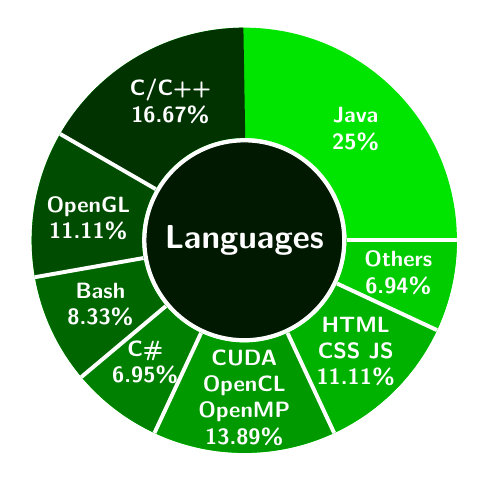
\begin{tikzpicture}[font=\sffamily\bfseries\large, 
     text=white, 
     border/.style={line width=14mm}]
\foreach \angle/\col [remember=\angle as \last (initially 0)] in 
    {360/green!90!black, 335/green!80!black, 295/green!70!black, 245/green!60!black, 220/green!50!black, 190/green!40!black, 150/green!30!black, 90/green!20!black}{    
		\draw[\col, border] (\last:2cm) 
             arc[start angle=\last, end angle=\angle, radius=2cm];
		\draw[white, line width=0.5mm] (\last:1.3)--++(\last:1.4);
}
\node[text width=2.1cm, align=center, font=\sffamily\bfseries\large, draw, circle, minimum width=2.5cm, white, fill=green!10!black] {Languages};
\node[text width=1.1cm, align=center, font=\sffamily\bfseries\footnotesize] at (45:2cm) 
    {Java 25\%};
\node[text width=1.1cm, align=center, font=\sffamily\bfseries\footnotesize] at (118:2cm) 
    {C/C++ 16.67\%};
\node[text width=1.1cm, align=center, font=\sffamily\bfseries\footnotesize] at (172:2cm) 
    {OpenGL 11.11\%};    
\node[text width=1.1cm, align=center, font=\sffamily\bfseries\footnotesize] at (204:2cm) 
    {Bash 8.33\%};  
\node[text width=1.1cm, align=center, font=\sffamily\bfseries\footnotesize] at (231:2cm) 
    {C\# 6.95\%};       
\node[text width=1.2cm, align=center, font=\sffamily\bfseries\footnotesize] at (270:2cm) 
    {CUDA OpenCL OpenMP 13.89\%};
\node[text width=1cm, align=center, font=\sffamily\bfseries\footnotesize] at (315:2cm) 
    {HTML CSS JS 11.11\%};
\node[text width=1cm, align=center, font=\sffamily\bfseries\footnotesize] at (348:2cm) 
    {Others 6.94\%};
\end{tikzpicture}
\end{document}
